% Figure from MATH 493 notes, section 55 (the action of Z/3Z on Z/7Z by x -> 2^k x). Added, not from lecture.
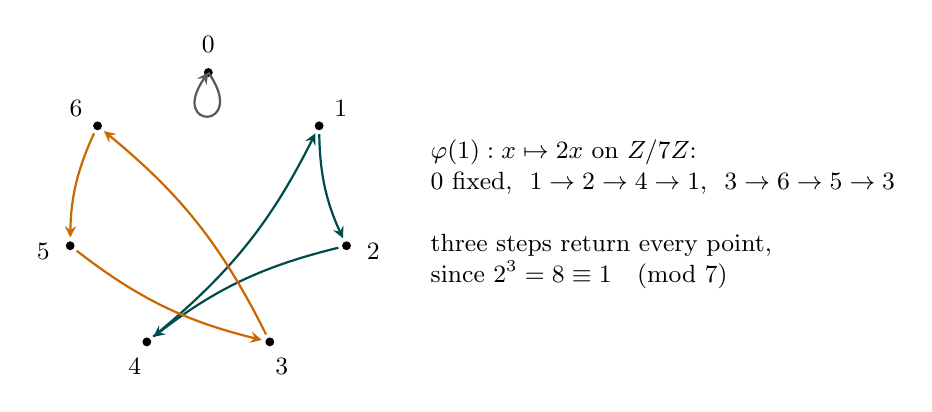
\begin{tikzpicture}[>=stealth, font=\small]
    \foreach \x in {0,...,6} { \coordinate (p\x) at ({90 - 360*\x/7}:1.8); }
    \foreach \x in {0,...,6} { \fill (p\x) circle (1.6pt); \node at ({90 - 360*\x/7}:2.15) {$\x$}; }
    \draw[->, thick, teal!60!black, shorten >=3pt, shorten <=3pt] (p1) to[bend right=12] (p2);
    \draw[->, thick, teal!60!black, shorten >=3pt, shorten <=3pt] (p2) to[bend right=12] (p4);
    \draw[->, thick, teal!60!black, shorten >=3pt, shorten <=3pt] (p4) to[bend right=12] (p1);
    \draw[->, thick, orange!80!black, shorten >=3pt, shorten <=3pt] (p3) to[bend right=12] (p6);
    \draw[->, thick, orange!80!black, shorten >=3pt, shorten <=3pt] (p6) to[bend right=12] (p5);
    \draw[->, thick, orange!80!black, shorten >=3pt, shorten <=3pt] (p5) to[bend right=12] (p3);
    \draw[->, thick, gray!70!black] (p0) .. controls +(-55:0.9) and +(-125:0.9) .. (p0);
    \node[font=\small, align=left, anchor=west] at (2.7,0.6) {$\varphi(1): x \mapsto 2x$ on $\mathbb{Z}/7\mathbb{Z}$:\\ $0$ fixed, \ $1 \to 2 \to 4 \to 1$, \ $3 \to 6 \to 5 \to 3$};
    \node[font=\small, align=left, anchor=west] at (2.7,-0.6) {three steps return every point,\\ since $2^3 = 8 \equiv 1 \pmod 7$};
\end{tikzpicture}
